\documentclass{beamer}
% Copyright 2015 by Do Phan Thuan

% Loại mẫu slice
%\usetheme{AnnArbor}
%\usetheme{Antibes}
\usetheme{Boadilla}
%\usetheme{CambridgeUS}
%\usetheme{Hannover}

% Ký tự tiếng Việt
\usepackage[utf8]{vietnam}
\usepackage[utf8]{inputenc}
% Công thức toán
\usepackage{amsmath,amsthm,amssymb,epsfig}
% Chèn ảnh
\usepackage{graphicx}
% Chèn đường dẫn 
\usepackage{url}

% Vẽ đồ thị
\usepackage{pgfplots}

% Insert code
\usepackage{listings}
\lstset{language=C++,
   %keywords={break,case,catch,continue,else,elseif,end,for,function,
   %   global,if,otherwise,persistent,return,switch,try,while},
   basicstyle=\ttfamily,
   keywordstyle=\color{blue},
   commentstyle=\color{red},
   stringstyle=\color{dkgreen},
   frame=lrtb,
   %frame=5 pt,
   numbers=left,
   numberstyle=\tiny\color{gray},
   stepnumber=1,
   numbersep=10pt,
   backgroundcolor=\color{white},
   tabsize=4,
   showspaces=false,
   showstringspaces=false}
% Tô mầu cho bảng
\usepackage{colortbl}


\usepackage{color}

\definecolor{dkgreen}{rgb}{0,0.6,0}
\definecolor{gray}{rgb}{0.5,0.5,0.5}
\definecolor{mauve}{rgb}{0.58,0,0.82}
  
\definecolor{Xanh}{rgb}{0,0.5,1}
\definecolor{Do}{rgb}{1,0.25,0}
\definecolor{Vang}{rgb}{1,1,0}
\definecolor{Datroi}{rgb}{0,0,1}
% Vẽ hình
\usepackage{tikz}
\usetikzlibrary{arrows,shapes}
% Vẽ mạch điện
\usepackage[siunitx,european resistors]{circuitikz}

% multirow
\usepackage{multirow}

\usepackage{pbox}

% Tô mầu cho bảng
\usepackage{colortbl}
\definecolor{Xanh}{rgb}{0,0.5,1}
\definecolor{Do}{rgb}{1,0.25,0}
\definecolor{Vang}{rgb}{1,1,0}
\definecolor{Datroi}{rgb}{0,0,1}

% Một vài ký hiệu thường dùng
\def\R{{\mathbb R}}
\def\N{{\mathbb N}}
\def\X{{\mathcal X}}
\def\Y{{\mathcal Y}}
\def\F{{\mathcal F}}
\def\P{{\mathcal P}}
\def\E{{\mathbb E}}
\def\I{{\mathbb I}}
\def\sign{{\rm sign}}

% Xác định khoảng dãn trong bảng
%\renewcommand\arraystretch{1.6}

% a few macros
\newcommand{\bi}{\begin{itemize}}
\newcommand{\ei}{\end{itemize}}
\newcommand{\ig}{\includegraphics}
\newcommand{\subt}[1]{{\footnotesize \color{subtitle} {#1}}}

% named colors
\definecolor{offwhite}{RGB}{249,242,215}
\definecolor{foreground}{RGB}{255,255,255}
\definecolor{background}{RGB}{24,24,24}
\definecolor{title}{RGB}{107,174,214}
\definecolor{gray}{RGB}{155,155,155}
\definecolor{subtitle}{RGB}{102,255,204}
\definecolor{hilight}{RGB}{22,155,104}
\definecolor{vhilight}{RGB}{255,111,207}
\definecolor{lolight}{RGB}{155,155,155}
%\definecolor{green}{RGB}{125,250,125}

% Minted
%\usepackage{minted}
%\usemintedstyle{monokai}
%\newminted{cpp}{fontsize=\footnotesize}

% Graph styles]

%gets rid of bottom navigation bars
\setbeamertemplate{footline}[frame number]{}

%gets rid of bottom navigation symbols
%\setbeamertemplate{navigation symbols}{}

%gets rid of footer
%will override 'frame number' instruction above
%comment out to revert to previous/default definitions
%\setbeamertemplate{footline}{}

% Tác giả, Tiêu đề, vân vân
\title[]{{\huge \bf Thương mại điện tử}\\
 \large Kinh doanh service thuật toán }

\author[]{
Nguyễn Tuấn Đạt\\% \inst{1} 
Nguyễn Hữu Hoàng \\
Đặng Quang Trung\\
}

\institute[]{
%\inst{1}% 
}

\logo{
\includegraphics[scale=0.04]{hust.jpg} \vspace{220pt}}

\begin{document}

\begin{frame}
\titlepage
\end{frame}

\begin{frame}{Nội dung}
\tableofcontents
\end{frame}

\begin{frame}{Thực trạng}
\section{ Đặt vấn đề}
\subsection{Thực trạng}
\bi 
\item Môi trường công nghệ hiện nay ở Việt Nam khá tụt hậu so với các nước trên thế giới?
\item Các kĩ sư có khả năng tốt về thuật toán chưa có nhiều môi trường làm việc ở Việt Nam?
\ei 
\end{frame}
\begin{frame}{Câu hỏi đặt ra}
Các kĩ sư Khoa học máy tính , Hệ thống thông tin đều được cung cấp các kiến thức rất bài bản về lý thuyết tối ưu, học máy, xử lý ngôn ngữ tự nhiền, tính toán  song song  ... \\
--> Tại sao chúng ta không đưa những thuật toán này ra thực tế. 
\begin{figure}
\begin{center}

\includegraphics[scale=0.08]{1.jpg}
\end{center}

\end{figure}
\end{frame}
\begin{frame}{Ý tưởng}
\begin{center}
\begin{figure}
\begin{center}

\includegraphics[scale=0.2]{2.jpg}
\end{center}

\end{figure}
\Large{"Bán Thuật Toán"} \\


\end{center} 
Vấn đề : Cạnh tranh Google,  Facebook ... \\ Doanh nghiệp làm phầm mềm truyền thống ...
\begin{figure}
\begin{center}

\includegraphics[scale=0.2]{4.jpg}
\end{center}

\end{figure}
\begin{figure}
\begin{center}

\includegraphics[scale=0.2]{6.png}
\end{center}

\end{figure}
\end{frame}
\begin{frame}{Mô hình làm phần mềm truyền thống}
\begin{enumerate}
\item Khảo sát, thu thập thông tin khách hàng Vd: tôi muốn làm một hệ gợi ý, tôi muốn một hệ thống tìm đường .
\item Phân tích yêu cầu 
\item Thiết kế 
\item Cài đặt bảo trì 
\end{enumerate}
\begin{figure}
\begin{center}

\includegraphics[scale=0.5]{3.jpg}
\end{center}

\end{figure}
\end{frame}
\begin{frame}{Bùng nổ Internet}
\begin{center}

\includegraphics[scale=0.2]{internet.jpg}
\end{center}
\begin{itemize}
\item Càng ngày tốc độ mạng càng nhanh.
\item Dữ liệu liên tục thay đổi nhanh
\end{itemize}

\end{frame}
\begin{frame}{Mô tả ý tưởng}
\subsection{Ý tưởng}
Bán thuật toán gồm:
\begin{itemize}
\item Thuật toán 
\item Khả năng tính toán 
\end{itemize}
Tức là: Cung cấp các hệ thống {\color{hilight}"Web Service"} thuật toán online hướng tới các khách hàng doạnh nghiệp cần yêu cầu thuật toán đặc thù.
\end{frame}
\begin{frame}
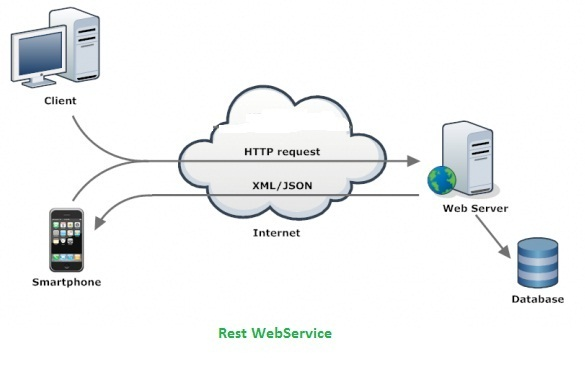
\includegraphics[scale=0.7]{R.jpg}
\end{frame}

\begin{frame}{Sản phẩm cung cấp}
\section{Sản phẩm}
\begin{enumerate}
\item Bài toán lập lịch trình, lập lịch sản xuất, tối ưu kho cảng, …

\item Bài toán xử lý ngôn ngữ tự nhiên: tách từ, phân tích quan điểm, từ điển....

\item Bài các bài toán nhận dạng: chữ viết, âm thanh, khuôn mặt,...
\item Bài toán gợi ý sản phẩm (sách, phim,...)
\item Bài toán khách hàng tự thiết lập(hệ trợ giúp quyết định, dự báo nhu cầu thị trường...)
\end{enumerate}
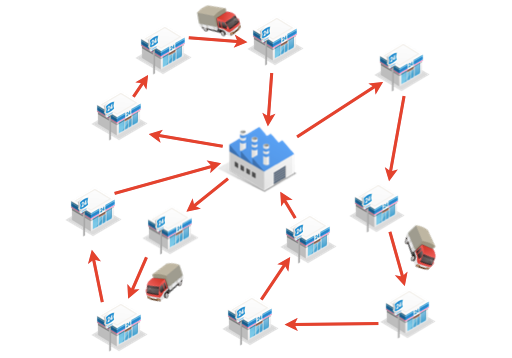
\includegraphics[scale=0.2]{VHR.png}
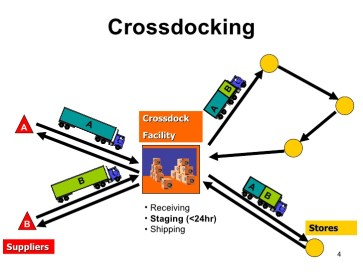
\includegraphics[scale=0.2]{CD.jpg}
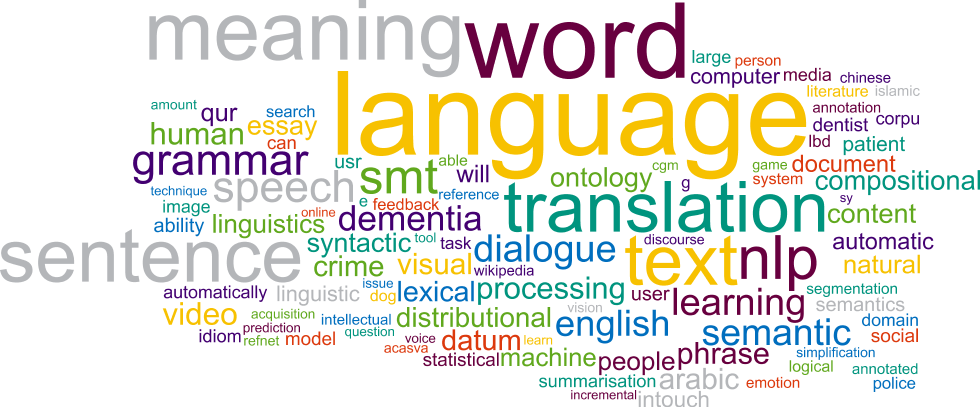
\includegraphics[scale=0.1]{NPL.png}

\includegraphics[scale=0.1]{ML.jpg}
\end{frame}
\begin{frame}{Khách hàng}
\section{Khách hàng hướng tới}
\begin{center}

\includegraphics[scale=0.2]{B2B.jpg}
\end{center}

\begin{itemize}
\item Các công ty giao vận cần tối ưu lịch trình.
\item Các công ty sản xuất cần lập lịch sản xuất, tối ưu kho cảng.
\item Các ứng dụng, website cần thêm các thao tác xử lý ngôn ngữ, phân tích quan điểm quan điểm của người dùng (chẳng hạn như qua bình luận, qua đánh giá sản phẩm,...)
\item Các ứng dụng cần các thao tác xử lý hình ảnh âm thanh, (như ứng dụng du lịch nhận dạng chữ qua hình ảnh và dịch luôn, các ứng dụng đọc tin tức bằng giọng nói,...)
\item Các website nhỏ mong muốn gợi ý sản phẩm tốt hơn cho khách hàng.
\item Các công ty yêu cầu các giải pháp đặc thù: dự báo thị trường, trợ giúp quyết định kinh doanh, ... 

\end{itemize}

\end{frame}
\begin{frame}{Tại sao ý tưởng lại có tiềm năng}
\section{Tính khả thi }
\begin{itemize}
\item Môi trường phát triển của start up
\item Nhu cầu của thị trường..
\item Tránh được mối lo cạnh tranh..
\item Tạo cơ hội đưa các bài toán nghiên cứu ra ứng dụng thực tế..
\end{itemize} 
\end{frame}
\begin{frame}{Mô tả cách thức hoạt động của hệ thống}
\section{Mô tả cách thức hoạt động của hệ thống}
\begin{center}
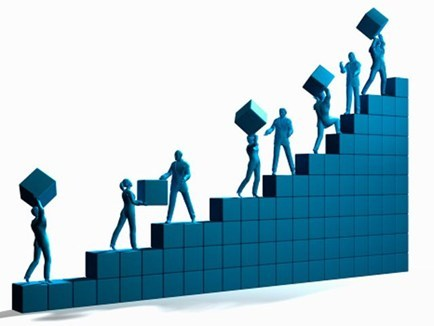
\includegraphics[scale=0.5]{TK.jpg}
\end{center}

\end{frame}
\begin{frame}{Giao diện hoạt động}

\subsection{Giao diện hoạt động}
Xây dựng website thương mại điện tử mà ở đó hàng hóa chính là các thuật toán. Khách hàng có thể tìm kiếm đặt hàng.\\

Trên website có thông tin mô tả về các api mà hệ thống cung cấp cũng như tài liệu hướng dẫn sử dụng, demo hệ thống v.v
\end{frame}
\begin{frame}{Quy trình hoạt động}
\begin{center}

\includegraphics[scale=0.4]{quytrinhhoatdong.png}\\
\end{center}
\end{frame}
\begin{frame}{Quy trình hoạt động}
\subsection{Quy trình hoạt động}
\begin{enumerate}
\item Người dùng đăng ký tài khoản trên website của công ty
\item Người dùng chọn sản phẩm muốn yêu cầu nhận key.
\item Web site cho phép người dùng chọn: key miễn phí, key trả phí bằng thẻ visa hoặc thẻ điện thoại . 
\item Người dùng theo đó chọn loại mình mong muốn và trả phí nếu có.
\item Mỗi khi sử dụng API của công ty, người dùng request lên server của công ty với đầu vào đúng như documentation mà công ty cung cấp, kèm theo key được cung cấp.
\item Phía server  kiểm tra key và dữ liệu. nếu key không cho phép tính năng này hoặc key hết hạn, hoặc dữ liệu không đúng, thì trả về thông báo tương ứng cho người dùng.
\item Nếu key và dữ liệu được chấp nhận, server xử lý và trả kết quả lại cho client. Nếu có thể xử lý ngay thời điểm đó thì trả lại luôn cho phía client. Nếu dữ liệu lớn và cần có thời gian lâu, server sẽ thông báo thời gian ước lượng cho phía client, tới thời điểm đó client request lên và nhận kết quả trả về. 

\end{enumerate}
\end{frame}

\begin{frame}{Quy trình đăng ký}
\begin{center}
\begin{figure}
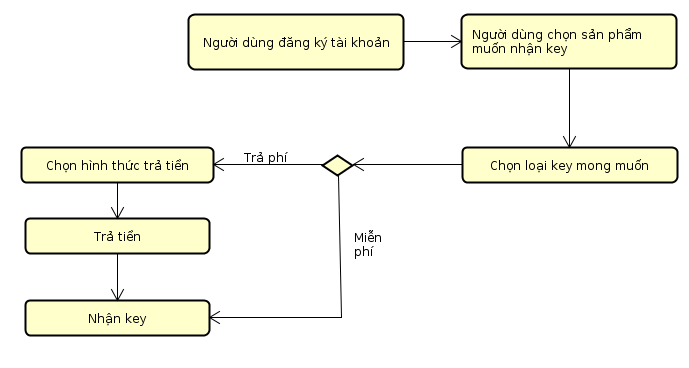
\includegraphics[scale=0.4]{dangky.png}
\end{figure}
\end{center}
\end{frame}

\begin{frame}{Quy trình sử dụng}
\begin{center}
\begin{figure}
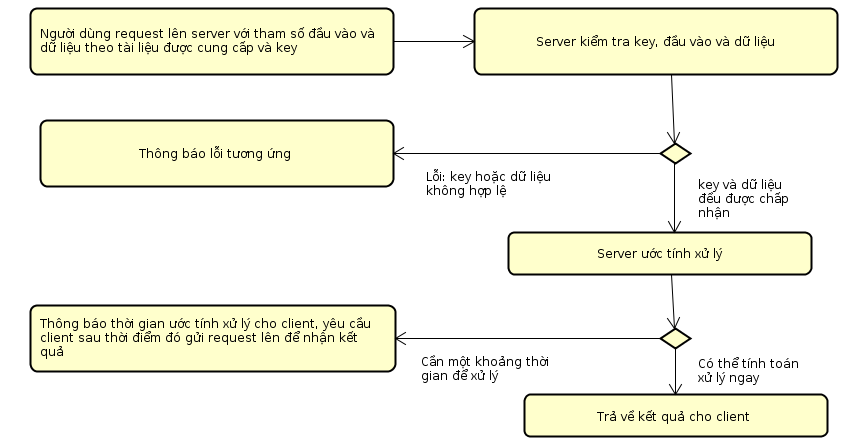
\includegraphics[scale=0.4]{sudung.png}
\end{figure}
\end{center}
\end{frame}

\begin{frame}{Giao dịch thanh toán}
\begin{center}

\includegraphics[scale=0.4]{giaodich.jpg}
\end{center}
\end{frame}
\begin{frame}{Giao dịch thanh toán}
\subsection{Giao dịch thanh toán}


Người dùng đăng ký tài khoản trên website của công ty và yêu cầu nhận key.\\
Công ty sẽ cung cấp hai loại key:
\begin{itemize}
\item key miễn phí: người dùng không cần trả phí, nhưng chỉ được dùng những tính năng nhất định với dữ liệu đầu vào nhỏ và lượng request hạn chế.
\item key trả tiền: có thể có nhiều loại key trả tiền khác nhau tương ứng với những gì mà khách hàng mong nuốn. Người dùng được dùng các tính năng tương ứng với dữ liệu và lượng request lớn. 
\end{itemize}
\end{frame}
\begin{frame}{Giao dịch thanh toán}
Hình thức thanh toán cho key trả tiền: \\
\begin{itemize}
\item Thông qua thẻ điện thoại, khi đó khách hàng sẽ cung cấp mã thẻ điện thoại của Viettel, VinaPhone cho công ty. Khách hàng nội địa có thể sử dụng hình thức này mà không cần tới thẻ Visa, Master.
\item Thông qua các loại thẻ Visa, Master. Thông qua các loại thẻ này, khách hàng quốc tế có thể sử dụng được dịch vụ của công ty.

\end{itemize}


\end{frame}
\begin{frame}{Giao dịch thanh toán}
Các key này có giới hạn về thời gian hoặc số lần sử dụng. Hết thời hạn, khách hàng có thể gia hạn thêm hoặc mua key khác. Khách hàng cũng có thể yêu cầu bổ sung thêm tính năng tương ứng với key. Đều cần trả thêm tiền.\\

Các công ty yêu cầu các bài toán đặc thù cần thiết kế giải pháp thì công ty sẽ thiết lập hợp đồng với họ, các chính sách và chi phí là theo thỏa thuận của hai bên.

\end{frame}
\begin{frame}{Marketing}
\begin{center}

\includegraphics[scale=0.7]{marketing.jpg}\\
\end{center}
\end{frame}
\begin{frame}{Marketing}
\section{Marketing}

\begin{itemize}
\item Công ty thực hiện quảng cáo qua Facebook và Google.

\item Mỗi năm công ty có các đợt khuyến mãi, trong đó cung cấp miễn phí một số lượng key professtional ra thị trường, để quảng bá cho sản phẩm của công ty.

\item Tại những thời điểm ban đầu, công ty cung cấp các ứng dụng trên nền web, app ứng dụng các giải pháp trên; thực hiện thử nghiệm các giải pháp tối ưu tại các đơn vị để gây tiếng vang, nâng cao hình ảnh và uy tín của công ty trên thị trường.


\end{itemize}

\end{frame}
\begin{frame}{Hậu mãi/ Bảo hành}
\begin{center}

\includegraphics[scale=0.5]{8.jpg}
\end{center}
\section{Hẫu mãi bảo hành}
\begin{itemize}
\item Khách hàng sử dụng key free cần tuân thủ các quy định và chính sách của công ty.

\item Khách hàng sử dụng key trả phí khi gặp trục trặc, vấn đề sẽ được các chuyên viên tham gia điều chỉnh, xử lý.

\item Khách hàng là các công ty có hợp đồng:
\begin{itemize}
\item Sẽ có các chuyên gia lành nghề tham gia khảo sát, thiết kế, triển khai vận hành.
\item Khi nào có trục trặc công ty sẽ cử chuyên gia đến xem xét và sửa chữa.
\end{itemize}
%	các chuyên gia sẽ tham gia quá trình khảo sát, thiết kế, triển khai vận hành; bất cứ khi nào có trục trặc sẽ được các chuyên viên hoặc chuyên gia trực tiếp khảo sát, xử lý.%
\end{itemize}
\end{frame}
\begin{frame}{Vấn đề bảo mật}
\begin{center}

\includegraphics[scale=0.2]{9.jpg}
\end{center}
\section{Bảo mật}
\begin{itemize}
\item Công ty sẽ có các chính sách bảo mật cho khách hàng:
\begin{itemize}
\item Khách hàng dùng key miễn phí sẽ có các khuyến cáo về bảo mật dữ liệu dữ liệu.
\item Khách hàng dùng key bản quyền hoặc có kí kết hợp đồng với công ty thì các dữ liệu khác hàng cung cấp sẽ đc công ty cam kết giữ bí mật theo yêu cầu của khách hàng(trong khoảng thời gian khách yêu cầu).
\end{itemize}
\item Vi phạm cam kết, công ty sẽ chịu phạt và bồi thường theo hợp đồng.
\end{itemize}
\end{frame}
\begin{frame}{Thách thức}
\section{Thách thức}
\textbf{Con người(Nhân lực):}
\begin{itemize}
\item Cần có đội ngũ có đội ngũ nhân viên có tri thức cao về học máy, xử lí dữ liệu lơn,khai phá dữ liệu,\ldots
\item Cần luôn tìm kiếm, thu hút những người có khả năng,đặc biệt là các bạn sinh viên có khả năng tốt và mong muốn phát triển công nghệ Việt Nam.
\end{itemize}
\textbf{Kinh phí:}
\begin{itemize}
\item Do nhu cầu cần tính toán và xử lí dữ liệu lớn nên cần có nguồn vốn để đầu tử cho máy móc(server)
\item Cần có chi phí quảng cáo cho các dịch vụ của công ty. 
\end{itemize}
\end{frame}
\begin{frame}{Giải pháp}
\section{Giải pháp}
\begin{itemize}
\item Ban đầu xây dựng các công nghê, thư viện public bởi cộng đồng và các công ty lớn như "google, facebook,..." public để áp dụng cho các thuật toán trên các mô hình được xây dựng và cung cấp api cho người dùng.
\item Khi có nguồn vốn sẽ tự xây dưng và phát triển thư viện riêng để áp dụng cho các bài toán.
\item Kêu gọi vốn đầu tư.
\end{itemize}
\end{frame}
\begin{frame}
\begin{center}

\includegraphics[scale=0.4]{thanks.jpg}\\
\end{center}
\end{frame}
\end{document}